\documentclass[11pt, fleqn]{article}

\usepackage[usenames,dvipsnames,svgnames,table]{xcolor}
\usepackage{amsmath}
\usepackage{amsfonts}
\usepackage[margin=1in]{geometry} % To set the margin widths
\usepackage{graphicx}
\usepackage{listings}
\usepackage{multirow}
\usepackage{tabularx}
\usepackage{varioref}
\usepackage[noabbrev,capitalize]{cleveref}
\usepackage[group-separator={,}]{siunitx}
\usepackage{subcaption}
\usepackage{titlesec}
\usepackage{lscape}
\usepackage{bm}
\usepackage[titletoc,toc,title]{appendix}

\lstset{
  frame=single,
  basicstyle=\ttfamily,% print whole listing small
  language=R,
  aboveskip=3mm,
  belowskip=3mm,
  showstringspaces=false,
  columns=flexible,
  numbers=none,
  commentstyle=\color{ForestGreen},
  stringstyle=\color{Maroon},
  breaklines=true,
  breakatwhitespace=true,
  tabsize=2,
  literate={<-}{{$\gets$}}1 {~}{{$\sim$}}1
}

\sisetup{output-exponent-marker=\textsc{e}}

\setlength{\parskip}{12pt} % Sets a blank line in between paragraphs
\setlength\parindent{0pt} % Sets the indent for each paragraph to zero

\begin{document}

\title{Machine Learning (41204-01)\\HW \#7}
\author{Will Clark and Matthew DeLio \\
\textsf{\{will.clark,mdelio\}@chicagobooth.edu} \\
University of Chicago Booth School of Business}
\date{\today}
\maketitle

\section{Data Summary}

The user that has rated the most video games is \textsf{U584295664}; he has rated 53 games. This user is an extreme outlier, as the median user rated only two games and only one other user rated more than 21 games. This behavior makes him approximately 22 standard deviations above the mean. We can see in \cref{fig:histo_users} just how extreme this outlier is (the maximum value is marked with a red line).

The game that has been rated most frequently is \textsf{I760611623}; it has been rated 200 times. This game is also an extreme outlier, as the median game has been rated three times and the next most-rated game was rated by only 102 users. The rating profile for this game puts it at approximately 15 standard deviations above the mean. We can see in \cref{fig:histo_games} how far from the center of the distribution this game is (the maximum value is again marked in red).

\begin{figure}
\centering
\begin{subfigure}[b]{0.49\textwidth}
\caption{by User}
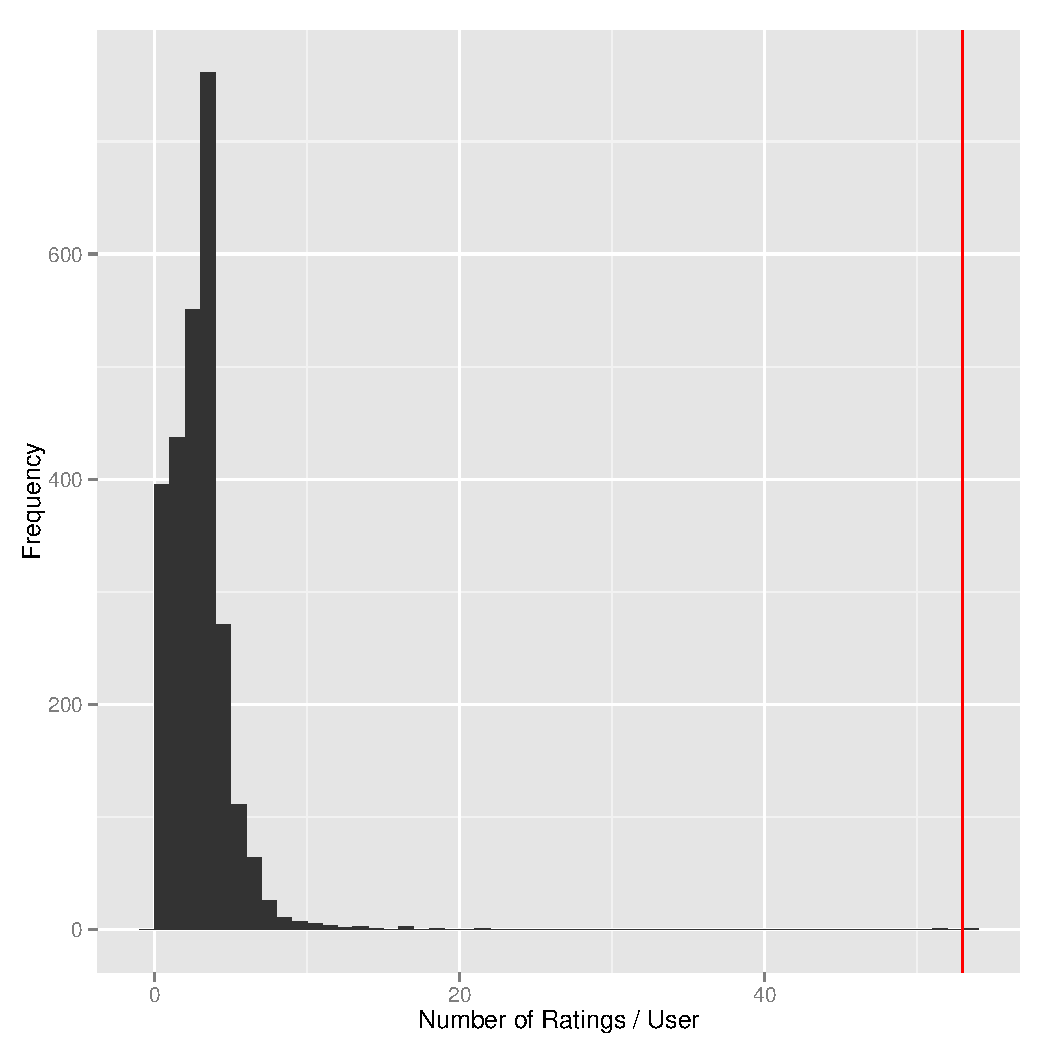
\includegraphics[width=\textwidth]{histo_users.pdf}
\label{fig:histo_users}
\end{subfigure}
\hfill
\begin{subfigure}[b]{0.49\textwidth}
\caption{by Game}
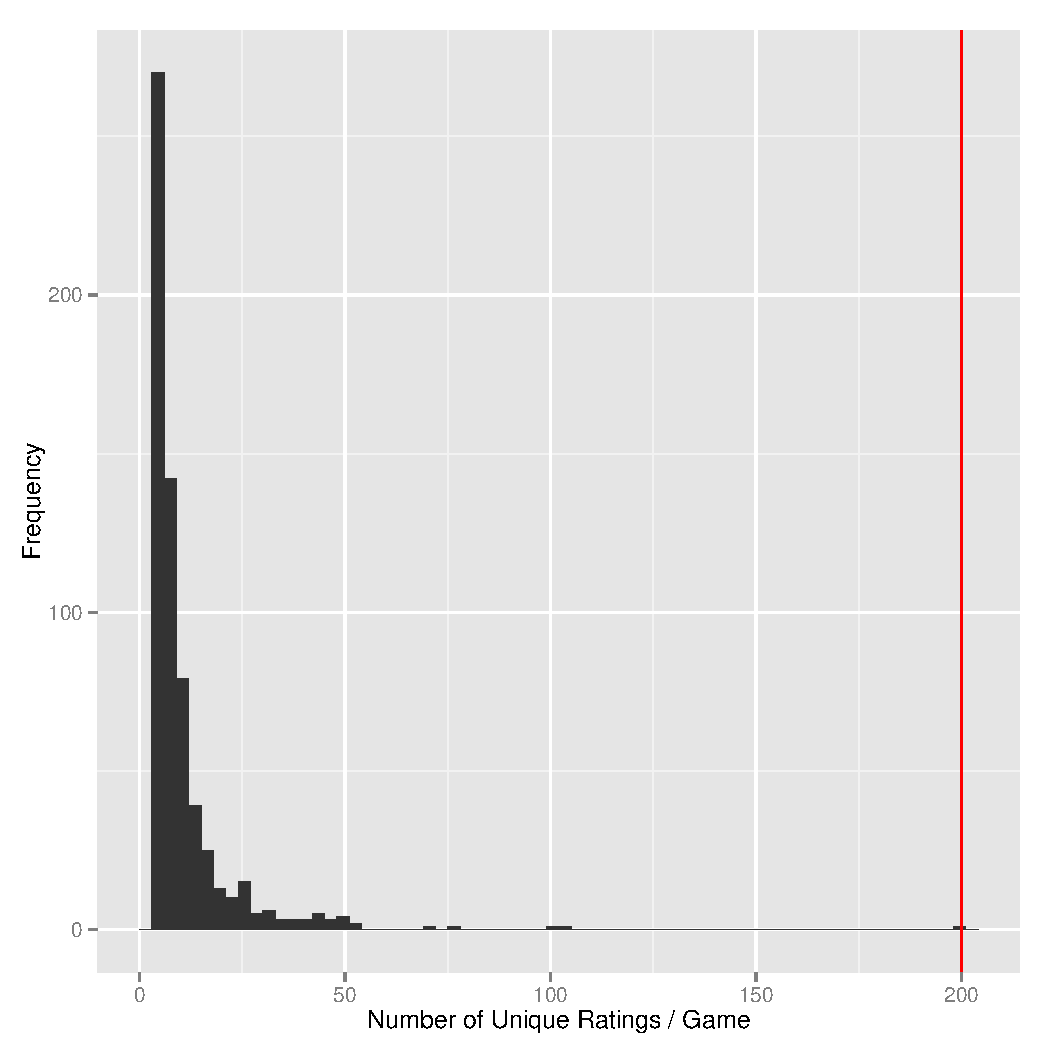
\includegraphics[width=\textwidth]{histo_games.pdf}
\label{fig:histo_games}
\end{subfigure}
\caption{Distribution of Rating Behavior}
\end{figure}

\section{User Similarity}
To find the user most similar to \textsf{U141954350}, we use RecommenderLab's similarity function.  To compute cosine similarity, we can simply feed the raw ratings data into the similarity function with our user in question, use the argument \textsf{method="cosine"}, and get a list of similarity scores between them and the others.

To compute Jaccard similarity, however, we had to "binarize" the ratings.  To do this, we first normalize the data, which attempts to reduce any user bias by row-centering the data (subtracts the user's mean score from each rating).  With this normalized data, we choose then to use the mean (now 0) as the cutoff between a binary 0/1.  This means that any score above the user's mean is a favorable score (\textsf{=1}), and any below, is a unfavorable (\textsf{=0}).  This binary data is then fed into the similarity function with the \textsf{method="jaccard"} argument which produces similarity scores between the user in question and the others.

%We attempted to use the \textsf{pearson} method, but ran into issues when calculating the similarity matrix (it returned only NAs).

The top 10 scores are listed in \cref{tab:top10}.  These show some good agreement between the two methods with the top 5 matching in exact order.  Furthermore, of the top 10 similar users, 9 appear in both lists.  The closest user to our user in question is \textsf{U887577623}

% latex table generated in R 3.2.2 by xtable 1.8-0 package
% Thu Nov 12 00:00:14 2015
\begin{table}[ht]
\centering
\caption{Top10 Users Similar to U141954350} 
\label{tab:top10}
\begin{tabular}{rll}
  \hline
 & Jaccard & Cosine \\ 
  \hline
1 & U887577623 & U887577623 \\ 
  2 & U067377044 & U067377044 \\ 
  3 & U906822504 & U906822504 \\ 
  4 & U293693102 & U293693102 \\ 
  5 & U506611447 & U506611447 \\ 
  6 & U246522212 & U722043563 \\ 
  7 & U457155042 & U246522212 \\ 
  8 & U574340933 & U606009295 \\ 
  9 & U606009295 & U943664133 \\ 
  10 & U943664133 & U457155042 \\ 
   \hline
\end{tabular}
\end{table}


\section{Recommendations}

To recommend a particular item to our user \textsf{U141954350} we utilize a ``popular'' recommender (see \vref{lst:code}).  We employ two methods for determining which item to recommend.
\begin{enumerate}
\item \textbf{Top-N List}\\Uses the recommender to produce a top 10 list based on the most popular items.
\item \textbf{Top Predicted Ratings}\\Predicts all ratings for the user, which can then be sorted to produce a top-10 list.
\end{enumerate}

Before beginning this analysis, we would have been surprised if these two lists were drastically different from one another --- in theory, they are supposed to produce the items that are ``best'' for the given user.  We find, however, that they produce completely different lists with drastically different predicted ratings (see \cref{tab:topn,tab:highest}).  Likely the algorithms work differently, one using user-similarity to predict a top list (Top-N List) and the other just producing top ratings with potentially low support (Top Predicted Ratings).  If this is the case, one would expect the Top-N List to represent a more robust list.  Therefore the item that we would recommend to the user is \textsf{I840620023}.

% latex table generated in R 3.2.2 by xtable 1.8-0 package
% Thu Nov 12 00:00:14 2015
\begin{table}[ht]
\centering
\caption{U141954350's Predicted Top 10 from Recommender} 
\label{tab:topn}
\begin{tabular}{rr}
  \hline
 & Predicted Rating \\ 
  \hline
I840620023 & 0.66 \\ 
  I040485258 & 0.56 \\ 
  I936489406 & 0.54 \\ 
  I659375008 & 0.49 \\ 
  I800474411 & 0.36 \\ 
  I357170215 & 0.34 \\ 
  I039793827 & 0.33 \\ 
  I232939121 & 0.33 \\ 
  I760611623 & 0.28 \\ 
  I962238428 & 0.17 \\ 
   \hline
\end{tabular}
\end{table}

% latex table generated in R 3.2.2 by xtable 1.8-0 package
% Thu Nov 12 00:41:14 2015
\begin{table}[ht]
\centering
\caption{U141954350's 10 Highest Rated Games} 
\label{tab:highest}
\begin{tabular}{rr}
  \hline
 & Predicted Rating \\ 
  \hline
I672894653 & 1.40 \\ 
  I599334538 & 1.21 \\ 
  I556596697 & 1.17 \\ 
  I298638212 & 1.11 \\ 
  I251454111 & 0.93 \\ 
  I315479240 & 0.85 \\ 
  I284106939 & 0.83 \\ 
  I938704872 & 0.82 \\ 
  I845782212 & 0.82 \\ 
  I803408952 & 0.78 \\ 
   \hline
\end{tabular}
\end{table}


\begin{appendices}

\clearpage
\section{Code Listings}
\lstinputlisting[label=lst:code, caption=Code for Homework, language=R]{../hw6.R}

\end{appendices}

\end{document}

% \input{.tex}

% \begin{figure}
%   \centering
%   \begin{subfigure}[b]{0.49\textwidth}
%     \caption{}
%     \includegraphics[width=\textwidth]{.pdf}
%     \label{fig:}
%   \end{subfigure}
%   \hfill
%   \begin{subfigure}[b]{0.49\textwidth}
%     \caption{}
%     \includegraphics[width=\textwidth]{.pdf}
%     \label{fig:}
%   \end{subfigure}
%   \caption{}
% \end{figure}

% \begin{figure}[!htb]
%   \centering
%   \caption{}
%   \includegraphics[scale=.5]{.pdf}
%   \label{fig:}
% \end{figure}

